\begin{figure}[htbp]
			\centering
			\resizebox{\textwidth}{!}{%
				\begin{tikzpicture}[>=stealth, line width=0.8pt, font=\small,
					nodo/.style  = {circle, fill=white, draw=black,
						inner sep=0pt, minimum size=5pt, line width=0.8pt},
					cint/.style  = {circle, fill=white, draw=black,
						inner sep=0pt, minimum size=6pt, line width=0.9pt},
					LI/.style    = {line width=1.0pt, black},
					frecciaLI/.style = {->, >=stealth, line width=0.9pt, black},
					richiam/.style = {thin, gray, dashed},
					]
					
					%% ── Parametri geometrici globali ─────────────────────────────────────────
					\def\L{1.50}     % ell (cm)
					\def\tw{0.20}    \def\thA{0.34}  \def\thR{0.28}
					\def\sr{0.07}    \def\bw{0.14}   \def\gw{0.26}
					
					%% Posizioni nodi (origine = A di ciascun pannello)
					\pgfmathsetmacro{\xB}{\L}
					\pgfmathsetmacro{\xG}{0.5*\L}
					\pgfmathsetmacro{\xE}{1.5*\L}
					\pgfmathsetmacro{\xH}{2.5*\L}
					\pgfmathsetmacro{\xF}{3.5*\L}
					\pgfmathsetmacro{\xC}{4*\L}
					\pgfmathsetmacro{\xD}{5*\L}
					
					%% Layout dei quattro pannelli
					\def\GAP{1.0}
					\def\HU{1.20}
					\def\VGbc{2.0}    % spazio verticale tra (b) e (c)
					\def\VGcd{1.4}    % spazio verticale tra (c) e (d)
					\pgfmathsetmacro{\XR}{\xD + \GAP}
					\pgfmathsetmacro{\YA}{-\HU - \VGbc}
					\def\YB{0}
					\pgfmathsetmacro{\YC}{-\HU - \VGbc}
					\pgfmathsetmacro{\YD}{-2*\HU - \VGbc - \VGcd}
					
					
					%% =========================================================================
					%% PANNELLO (a) — DATI REALI: cedimento s_A, distorsioni varrho_v, varrho_theta in G
					%% =========================================================================
					\begin{scope}[xshift=0cm, yshift=\YA cm]
						
						%% ── Trave ────────────────────────────────────────────────────────────
						\draw[line width=2.2pt](0,0)--(\xD,0);
						
						%% ── Fibra inferiore ──────────────────────────────────────────────────
						\draw[line width=0.6pt, dashed, gray!55](0,-0.13)--(\xD,-0.13);
						
						%% ── Etichette nodi ───────────────────────────────────────────────────
						\node[above=0.04]at(0,0){$A$};
						%\node[right=0.04]at(\xG,0.04){$G$};
						\node[above=0.04]at(\xB,0){$B$};
						\node[above=0.04]at(\xE,0){$E$};
						\node[above=0.04]at(\xH,0){$H$};
						\node[above=0.04]at(\xF,0){$F$};
						\node[above=0.04]at(\xC,0){$C$};
						\node[above=0.04]at(\xD,0){$D$};
						
						%% ── Etichetta G con freccia di richiamo (zona affollata dalle distorsioni) ──
						\coordinate (Glab) at (\xG, -0.85);
						\draw[->, line width=0.4pt, gray!70] (Glab) -- (\xG, -0.05);
						\node[font=\small] at (Glab){$G$};
						
						%% ── Cerniera A ───────────────────────────────────────────────────────
						\draw(0,0)--++(-\tw,-\thA)--++(2*\tw,0)--cycle;
						\draw(-\gw,-\thA)--(\gw,-\thA);
						\foreach \x in {-0.20,-0.10,0,0.10,0.20}
						\draw[thin](\x,-\thA)--++(-.07,-.09);
						\node[nodo]at(0,0){};
						
						%% ── Appoggio B (doppio rullo) ────────────────────────────────────────
						\draw(\xB,0)--++(-\tw,-\thR)--++(2*\tw,0)--cycle;
						\draw(\xB-\gw,-\thR)--(\xB+\gw,-\thR);
						\draw(\xB-\bw,-\thR-0.10)circle(2pt);
						\draw(\xB+\bw,-\thR-0.10)circle(2pt);
						\draw(\xB-\gw,-\thR-0.20)--(\xB+\gw,-\thR-0.20);
						\foreach \x in {-0.20,-0.10,0,0.10,0.20}
						\draw[thin](\xB+\x,-\thR-0.20)--++(-.07,-.09);
						\fill[white](\xB-\sr,0)arc(180:360:\sr)--cycle;
						\draw(\xB-\sr,0)arc(180:360:\sr);
						
						%% ── Appoggio C (doppio rullo) ────────────────────────────────────────
						\draw(\xC,0)--++(-\tw,-\thR)--++(2*\tw,0)--cycle;
						\draw(\xC-\gw,-\thR)--(\xC+\gw,-\thR);
						\draw(\xC-\bw,-\thR-0.10)circle(2pt);
						\draw(\xC+\bw,-\thR-0.10)circle(2pt);
						\draw(\xC-\gw,-\thR-0.20)--(\xC+\gw,-\thR-0.20);
						\foreach \x in {-0.20,-0.10,0,0.10,0.20}
						\draw[thin](\xC+\x,-\thR-0.20)--++(-.07,-.09);
						\fill[white](\xC-\sr,0)arc(180:360:\sr)--cycle;
						\draw(\xC-\sr,0)arc(180:360:\sr);
						
						%% ── Carrello D ───────────────────────────────────────────────────────
						\draw(\xD,0)--++(-\tw,-\thR)--++(2*\tw,0)--cycle;
						\draw(\xD-\gw,-\thR)--(\xD+\gw,-\thR);
						\draw(\xD-\bw,-\thR-0.10)circle(2pt);
						\draw(\xD+\bw,-\thR-0.10)circle(2pt);
						\draw(\xD-\gw,-\thR-0.20)--(\xD+\gw,-\thR-0.20);
						\foreach \x in {-0.20,-0.10,0,0.10,0.20}
						\draw[thin](\xD+\x,-\thR-0.20)--++(-.07,-.09);
						\node[nodo]at(\xD,0){};
						
						%% ── Cerniere interne E, F ────────────────────────────────────────────
						\node[cint]at(\xE,0){};
						\node[cint]at(\xF,0){};
						
						%% ═════════════════════════════════════════════════════════════════════
						%% DATI REALI
						%% ═════════════════════════════════════════════════════════════════════
						
						%% ── Cedimento verticale s_A in A: freccia verso il basso ─────────────
						\def\Sh{0.65}
						\draw[->, line width=0.8pt]
						(0, -\thA-\gw-0.05) -- (0, -\thA-\gw-0.05-\Sh);
						\node[left, font=\footnotesize]
						at (-0.06, -\thA-\gw-0.05-\Sh/2){$\bar s_A$};
						
						%% ── Distorsione trasversale varrho_v in G: due frecce verticali ──────
						%% contrapposte sui lembi G^- e G^+, lembo destro che scende rispetto
						%% al sinistro (concorde con T>0 orario)
						\def\dG{0.04}    % piccolo offset orizzontale per separare i lembi
						\def\fv{0.40}    % lunghezza freccia
						%% lembo sinistro (G^-): verso l'alto
						\draw[->, line width=0.7pt]
						(\xG-\dG, 0.10) -- (\xG-\dG, 0.10+\fv);
						%% lembo destro (G^+): verso il basso
						\draw[->, line width=0.7pt]
						(\xG+\dG, 0.10) -- (\xG+\dG, 0.10-\fv-0.10);
						\node[font=\footnotesize, left]
						at (\xG-\dG+0.06, 0.30+\fv/2){$\bar\varrho_v$};
						
						%				%% ── Rotazione relativa varrho_theta in G: due archetti contrapposti ──
						%				\def\rA{0.30}    % raggio archetti
						%				\draw[->, line width=0.6pt]
						%				(\xG+\dG+\rA, 0) arc (0:120:\rA);
						%				\draw[->, line width=0.6pt]
						%				(\xG-\dG-\rA, 0) arc (180:60:\rA);
						%				\node[font=\footnotesize, above]
						%				at (\xG, \rA+0.08){$\bar\varrho_\vartheta$};
						
						%% ── Rotazione relativa varrho_theta in G: due semiarchi ──────────────
						%% stile coppia interna: semiarco a sinistra di G^- (gira da 270 a 90),
						%% semiarco a destra di G^+ (gira da -90 a 90)
						\def\rA{0.18}    % raggio semiarchi (come nell'esempio)
						\draw[->, line width=0.85pt]
						(\xG-\dG-0.14, -\rA) arc (270:90:\rA);
						\draw[<-, line width=0.85pt]
						(\xG+\dG+0.14,  \rA) arc (90:-90:\rA);
						\node[right=0.0, font=\footnotesize]
						at (\xG+\dG-0.04, +0.4){$\bar\varrho_\vartheta$};
						
						
						%% ── Etichetta pannello ───────────────────────────────────────────────
						\node[font=\small,below=0.05]at(0.5*\xD,-1.40)
						{(a) Sistema reale: dati cinematici};
						
					\end{scope}
					
					
					%% =========================================================================
					%% PANNELLO (b) — SISTEMA VIRTUALE: F^*=1 in H, reazioni V_A^*, V_B^*, V_C^*, V_D^*
					%% =========================================================================
					\begin{scope}[xshift=\XR cm, yshift=\YB cm]
						
						%% ── Trave ────────────────────────────────────────────────────────────
						\draw[line width=2.2pt](0,0)--(\xD,0);
						
						%% ── Fibra inferiore ──────────────────────────────────────────────────
						\draw[line width=0.6pt, dashed, gray!55](0,-0.13)--(\xD,-0.13);
						
						%% ── Etichette nodi ───────────────────────────────────────────────────
						\node[above=0.04]at(0,0){$A$};
						\node[above=0.04]at(\xG,0){$G$};
						\node[above=0.04]at(\xB,0){$B$};
						\node[above=0.04]at(\xE,0){$E$};
						\node[below=0.04]at(\xH,0){$H$};
						\node[above=0.04]at(\xF,0){$F$};
						\node[above=0.04]at(\xC,0){$C$};
						\node[above=0.04]at(\xD,0){$D$};
						
						%% ── Cerniera A ───────────────────────────────────────────────────────
						\draw(0,0)--++(-\tw,-\thA)--++(2*\tw,0)--cycle;
						\draw(-\gw,-\thA)--(\gw,-\thA);
						\foreach \x in {-0.20,-0.10,0,0.10,0.20}
						\draw[thin](\x,-\thA)--++(-.07,-.09);
						\node[nodo]at(0,0){};
						
						%% ── Appoggio B (doppio rullo) ────────────────────────────────────────
						\draw(\xB,0)--++(-\tw,-\thR)--++(2*\tw,0)--cycle;
						\draw(\xB-\gw,-\thR)--(\xB+\gw,-\thR);
						\draw(\xB-\bw,-\thR-0.10)circle(2pt);
						\draw(\xB+\bw,-\thR-0.10)circle(2pt);
						\draw(\xB-\gw,-\thR-0.20)--(\xB+\gw,-\thR-0.20);
						\foreach \x in {-0.20,-0.10,0,0.10,0.20}
						\draw[thin](\xB+\x,-\thR-0.20)--++(-.07,-.09);
						\fill[white](\xB-\sr,0)arc(180:360:\sr)--cycle;
						\draw(\xB-\sr,0)arc(180:360:\sr);
						
						%% ── Appoggio C (doppio rullo) ────────────────────────────────────────
						\draw(\xC,0)--++(-\tw,-\thR)--++(2*\tw,0)--cycle;
						\draw(\xC-\gw,-\thR)--(\xC+\gw,-\thR);
						\draw(\xC-\bw,-\thR-0.10)circle(2pt);
						\draw(\xC+\bw,-\thR-0.10)circle(2pt);
						\draw(\xC-\gw,-\thR-0.20)--(\xC+\gw,-\thR-0.20);
						\foreach \x in {-0.20,-0.10,0,0.10,0.20}
						\draw[thin](\xC+\x,-\thR-0.20)--++(-.07,-.09);
						\fill[white](\xC-\sr,0)arc(180:360:\sr)--cycle;
						\draw(\xC-\sr,0)arc(180:360:\sr);
						
						%% ── Carrello D ───────────────────────────────────────────────────────
						\draw(\xD,0)--++(-\tw,-\thR)--++(2*\tw,0)--cycle;
						\draw(\xD-\gw,-\thR)--(\xD+\gw,-\thR);
						\draw(\xD-\bw,-\thR-0.10)circle(2pt);
						\draw(\xD+\bw,-\thR-0.10)circle(2pt);
						\draw(\xD-\gw,-\thR-0.20)--(\xD+\gw,-\thR-0.20);
						\foreach \x in {-0.20,-0.10,0,0.10,0.20}
						\draw[thin](\xD+\x,-\thR-0.20)--++(-.07,-.09);
						\node[nodo]at(\xD,0){};
						
						%% ── Cerniere interne E, F ────────────────────────────────────────────
						\node[cint]at(\xE,0){};
						\node[cint]at(\xF,0){};
						
						%% ═════════════════════════════════════════════════════════════════════
						%% SISTEMA VIRTUALE
						%% ═════════════════════════════════════════════════════════════════════
						
						%% ── Forza unitaria F*=1 in H verso il basso ──────────────────────────
						\def\Fh{0.85}    % altezza freccia carico
						\draw[->, line width=1.0pt]
						(\xH, \Fh) -- (\xH, 0.05);
						\node[above, font=\small] at (\xH, 0.9*\Fh){$F^{*}=1$};
						
						%% ── Reazioni alle estremità (frecce sotto la struttura, valori) ──────
						\def\Rh{0.55}    % altezza grafica delle frecce di reazione
						\def\Rqd{-\thA-\gw-0.20}    % quota di partenza sotto i vincoli (cerniera A)
						\def\Rqr{-\thR-\gw-0.20}    % quota di partenza sotto i vincoli (carrelli)
						
						%% V_A^* = -1/4 (freccia verso il basso, etichetta sotto la punta, centrata)
						\draw[->, line width=0.85pt]
						(0, \Rqd) -- (0, \Rqd-\Rh);
						\node[below, font=\footnotesize]
						at (0, \Rqd-\Rh){$V_A^{*}=\tfrac{1}{4}$};
						
						%% V_B^* = +3/4 (freccia verso l'alto, etichetta a destra)
						\draw[->, line width=0.85pt]
						(\xB, \Rqr-\Rh) -- (\xB, \Rqr);
						\node[right, font=\footnotesize]
						at (\xB+0.05, \Rqr-0.5*\Rh){$V_B^{*}=\tfrac{3}{4}$};
						
						%% V_C^* = +3/4 (freccia verso l'alto, etichetta a sinistra)
						\draw[->, line width=0.85pt]
						(\xC, \Rqr-\Rh) -- (\xC, \Rqr);
						\node[left, font=\footnotesize]
						at (\xC-0.05, \Rqr-0.5*\Rh){$V_C^{*}=\tfrac{3}{4}$};
						
						%% V_D^* = -1/4 (freccia verso il basso, etichetta sotto la punta, centrata)
						\draw[->, line width=0.85pt]
						(\xD, \Rqr) -- (\xD, \Rqr-\Rh);
						\node[below, font=\footnotesize]
						at (\xD, \Rqr-\Rh){$V_D^{*}=\tfrac{1}{4}$};
						
						
						%% ── Etichetta pannello ───────────────────────────────────────────────
						\node[font=\small,below=0.05]at(0.5*\xD,-1.40)
						{(b) Sistema virtuale};
						
					\end{scope}
					%% =========================================================================
					%% PANNELLO (c) — DIAGRAMMA DEL TAGLIO T*
					%% =========================================================================
					\begin{scope}[xshift=\XR cm, yshift=\YC cm]
						
						%% ── Altezza grafica del diagramma ────────────────────────────────────
						\def\hT{1.20}
						
						%% Quote dei quattro tratti
						\pgfmathsetmacro{\yAB}{-0.25*\hT}
						\pgfmathsetmacro{\yBH}{ 0.50*\hT}
						\pgfmathsetmacro{\yHC}{-0.50*\hT}
						\pgfmathsetmacro{\yCD}{ 0.25*\hT}
						
						%% Centri orizzontali e verticali dei rettangoli (precalcolati)
						\pgfmathsetmacro{\xMab}{0.5*\xB}
						\pgfmathsetmacro{\xMbh}{0.5*(\xB+\xH)}
						\pgfmathsetmacro{\xMhc}{0.5*(\xH+\xC)}
						\pgfmathsetmacro{\xMcd}{0.5*(\xC+\xD)}
						\pgfmathsetmacro{\yMab}{0.5*\yAB}
						\pgfmathsetmacro{\yMbh}{0.5*\yBH}
						\pgfmathsetmacro{\yMhc}{0.5*\yHC}
						\pgfmathsetmacro{\yMcd}{0.5*\yCD}
						
						%% 	═════════════════════════════════════════════════════════════════════
						%% DIAGRAMMA (disegnato per primo)
						%% ═════════════════════════════════════════════════════════════════════
						
						\draw[line width=1.0pt, fill=black!8] (0,0) -- (0,\yAB)
						-- (\xB,\yAB) -- (\xB,0) -- cycle;
						\draw[line width=1.0pt, fill=black!8] (\xB,0) -- (\xB,\yBH)
						-- (\xH,\yBH) -- (\xH,0) -- cycle;
						\draw[line width=1.0pt, fill=black!8] (\xH,0) -- (\xH,\yHC)
						-- (\xC,\yHC) -- (\xC,0) -- cycle;
						\draw[line width=1.0pt, fill=black!8] (\xC,0) -- (\xC,\yCD)
						-- (\xD,\yCD) -- (\xD,0) -- cycle;
						
						% 			%% Simboli oplus/ominus al centro dei rettangoli, in cerchio bianco
						\node[circle, draw=black, fill=white, inner sep=0pt, minimum size=8pt,
						line width=0.6pt, font=\scriptsize]
						at (\xMab,\yMab) {$-$};
						\node[circle, draw=black, fill=white, inner sep=0pt, minimum size=8pt,
						line width=0.6pt, font=\scriptsize]
						at (\xMbh,\yMbh) {$+$};
						\node[circle, draw=black, fill=white, inner sep=0pt, minimum size=8pt,
						line width=0.6pt, font=\scriptsize]
						at (\xMhc,\yMhc) {$-$};
						\node[circle, draw=black, fill=white, inner sep=0pt, minimum size=8pt,
						line width=0.6pt, font=\scriptsize]
						at (\xMcd,\yMcd) {$+$};
						
						
						%% Etichette dei moduli (fuori dai rettangoli)
						\node[below, font=\footnotesize] at (\xMab,\yAB) {$\tfrac{1}{4}$};
						\node[left, font=\footnotesize] at (\xB,\yBH) {$\tfrac{1}{2}$};
						\node[left, font=\footnotesize] at (\xH,\yHC) {$\tfrac{1}{2}$};
						\node[left, font=\footnotesize] at (\xC,\yCD) {$\tfrac{1}{4}$};
						
						%% ═════════════════════════════════════════════════════════════════════
						%% STRUTTURA (sopra il diagramma)
						%% ═════════════════════════════════════════════════════════════════════
						
						%% Trave
						\draw[line width=2.2pt] (0,0) -- (\xD,0);
						
						%% Etichette nodi
						% 			\node[above=0.04] at (0,0)   {$A$};
						% 			\node[left] at (\xB,0.3) {$B$};
						% 			\node[below=0.04] at (\xE,0) {$E$};
						% 			\node[right] at (\xH,0.3) {$H$};
						% 			\node[above=0.04] at (\xF,0) {$F$};
						% 			\node[left] at (\xC,0.3) {$C$};
						% 			\node[right] at (\xD,0.3) {$D$};
						
						%% Cerniera A
						\draw (0,0) -- ++(-\tw,-\thA) -- ++(2*\tw,0) -- cycle;
						\draw (-\gw,-\thA) -- (\gw,-\thA);
						\foreach \x in {-0.20,-0.10,0,0.10,0.20}
						\draw[thin] (\x,-\thA) -- ++(-.07,-.09);
						\node[nodo] at (0,0) {};
						
						%% Appoggio B
						\draw (\xB,0) -- ++(-\tw,-\thR) -- ++(2*\tw,0) -- cycle;
						\draw (\xB-\gw,-\thR) -- (\xB+\gw,-\thR);
						\draw (\xB-\bw,-\thR-0.10) circle (2pt);
						\draw (\xB+\bw,-\thR-0.10) circle (2pt);
						\draw (\xB-\gw,-\thR-0.20) -- (\xB+\gw,-\thR-0.20);
						\foreach \x in {-0.20,-0.10,0,0.10,0.20}
						\draw[thin] (\xB+\x,-\thR-0.20) -- ++(-.07,-.09);
						\fill[white] (\xB-\sr,0) arc (180:360:\sr) -- cycle;
						\draw (\xB-\sr,0) arc (180:360:\sr);
						
						%% Appoggio C
						\draw (\xC,0) -- ++(-\tw,-\thR) -- ++(2*\tw,0) -- cycle;
						\draw (\xC-\gw,-\thR) -- (\xC+\gw,-\thR);
						\draw (\xC-\bw,-\thR-0.10) circle (2pt);
						\draw (\xC+\bw,-\thR-0.10) circle (2pt);
						\draw (\xC-\gw,-\thR-0.20) -- (\xC+\gw,-\thR-0.20);
						\foreach \x in {-0.20,-0.10,0,0.10,0.20}
						\draw[thin] (\xC+\x,-\thR-0.20) -- ++(-.07,-.09);
						\fill[white] (\xC-\sr,0) arc (180:360:\sr) -- cycle;
						\draw (\xC-\sr,0) arc (180:360:\sr);
						
						%% Carrello D
						\draw (\xD,0) -- ++(-\tw,-\thR) -- ++(2*\tw,0) -- cycle;
						\draw (\xD-\gw,-\thR) -- (\xD+\gw,-\thR);
						\draw (\xD-\bw,-\thR-0.10) circle (2pt);
						\draw (\xD+\bw,-\thR-0.10) circle (2pt);
						\draw (\xD-\gw,-\thR-0.20) -- (\xD+\gw,-\thR-0.20);
						\foreach \x in {-0.20,-0.10,0,0.10,0.20}
						\draw[thin] (\xD+\x,-\thR-0.20) -- ++(-.07,-.09);
						\node[nodo] at (\xD,0) {};
						
						%% Cerniere interne E, F
						\node[cint] at (\xE,0) {};
						\node[cint] at (\xF,0) {};
						
						%% Etichetta pannello
						
						\node[font=\small, below=0.05] at (0.5*\xD, \yHC-0.55)
						{(c) Diagramma di $T^{*}$};
						
					\end{scope}
					%			
					%% =========================================================================
					%% PANNELLO (d) — DIAGRAMMA DEL MOMENTO M*
					%% Andamento triangolato con valori notevoli:
					%%   M*(A) = 0,  M*(B) = -ell/4 (top tese), 
					%%   M*(E) = 0 (cerniera), M*(H) = +ell/2 (bottom tese), 
					%%   M*(F) = 0 (cerniera), M*(C) = -ell/4 (top tese), M*(D) = 0
					%% =========================================================================
					\begin{scope}[xshift=\XR cm, yshift=\YD cm]
						
						%% ── Altezza grafica del diagramma ────────────────────────────────────
						%% Convenzione europea: M positivo verso il basso (lato fibre tese),
						%% M negativo verso l'alto.
						\def\hM{0.80}    % altezza grafica per |M| = ell
						
						%% Quote ai punti notevoli (segno invertito: M>0 -> y<0, M<0 -> y>0)
						\pgfmathsetmacro{\yMb}{ 0.25*\hM*\L}    % M(B) = -ell/4 -> sopra
						\pgfmathsetmacro{\yMe}{ 0          }    % M(E) = 0
						\pgfmathsetmacro{\yMh}{-0.50*\hM*\L}    % M(H) = +ell/2 -> sotto
						\pgfmathsetmacro{\yMf}{ 0          }    % M(F) = 0
						\pgfmathsetmacro{\yMc}{ 0.25*\hM*\L}    % M(C) = -ell/4 -> sopra
						
						%% ═════════════════════════════════════════════════════════════════════
						%% DIAGRAMMA (disegnato per primo)
						%% ═════════════════════════════════════════════════════════════════════
						
						%% Tratto AB: lineare da 0 a yMb (sopra l'asse)
						\draw[line width=1.0pt, fill=black!8]
						(0,0) -- (\xB,\yMb) -- (\xB,0) -- cycle;
						
						%% Tratto BE: lineare da yMb a 0 (chiude in E)
						\draw[line width=1.0pt, fill=black!8]
						(\xB,0) -- (\xB,\yMb) -- (\xE,0) -- cycle;
						
						%% Tratto EH: lineare da 0 a yMh (sotto l'asse)
						\draw[line width=1.0pt, fill=black!8]
						(\xE,0) -- (\xH,\yMh) -- (\xH,0) -- cycle;
						
						%% Tratto HF: lineare da yMh a 0 (chiude in F)
						\draw[line width=1.0pt, fill=black!8]
						(\xH,0) -- (\xH,\yMh) -- (\xF,0) -- cycle;
						
						%% Tratto FC: lineare da 0 a yMc (sopra l'asse)
						\draw[line width=1.0pt, fill=black!8]
						(\xF,0) -- (\xC,\yMc) -- (\xC,0) -- cycle;
						
						%% Tratto CD: lineare da yMc a 0
						\draw[line width=1.0pt, fill=black!8]
						(\xC,0) -- (\xC,\yMc) -- (\xD,0) -- cycle;
						
						%% Etichette dei valori notevoli (fuori dai poligoni)
						\node[above, font=\footnotesize] at (\xB,\yMb) {$\tfrac{\ell}{4}$};
						\node[below, font=\footnotesize] at (\xH,\yMh) {$\tfrac{\ell}{2}$};
						\node[above, font=\footnotesize] at (\xC,\yMc) {$\tfrac{\ell}{4}$};
						
						%% ═════════════════════════════════════════════════════════════════════
						%% STRUTTURA (sopra il diagramma)
						%% ═════════════════════════════════════════════════════════════════════
						
						%% Trave
						\draw[line width=2.2pt] (0,0) -- (\xD,0);
						
						%% Fibra inferiore (linea di riferimento per il segno di M)
						\draw[line width=0.6pt, dashed, gray!55] (0,-0.13) -- (\xD,-0.13);
						
						%% Etichette nodi
						%	\node[above=0.04] at (0,0)   {$A$};
						%	\node[above=0.04] at (\xB,0) {$B$};
						%	\node[above=0.04] at (\xE,0) {$E$};
						%	\node[above=0.04] at (\xH,0) {$H$};
						%	\node[above=0.04] at (\xF,0) {$F$};
						%	\node[above=0.04] at (\xC,0) {$C$};
						%	\node[above=0.04] at (\xD,0) {$D$};
						
						%% Cerniera A
						\draw (0,0) -- ++(-\tw,-\thA) -- ++(2*\tw,0) -- cycle;
						\draw (-\gw,-\thA) -- (\gw,-\thA);
						\foreach \x in {-0.20,-0.10,0,0.10,0.20}
						\draw[thin] (\x,-\thA) -- ++(-.07,-.09);
						\node[nodo] at (0,0) {};
						
						%% Appoggio B
						\draw (\xB,0) -- ++(-\tw,-\thR) -- ++(2*\tw,0) -- cycle;
						\draw (\xB-\gw,-\thR) -- (\xB+\gw,-\thR);
						\draw (\xB-\bw,-\thR-0.10) circle (2pt);
						\draw (\xB+\bw,-\thR-0.10) circle (2pt);
						\draw (\xB-\gw,-\thR-0.20) -- (\xB+\gw,-\thR-0.20);
						\foreach \x in {-0.20,-0.10,0,0.10,0.20}
						\draw[thin] (\xB+\x,-\thR-0.20) -- ++(-.07,-.09);
						\fill[white] (\xB-\sr,0) arc (180:360:\sr) -- cycle;
						\draw (\xB-\sr,0) arc (180:360:\sr);
						
						%% Appoggio C
						\draw (\xC,0) -- ++(-\tw,-\thR) -- ++(2*\tw,0) -- cycle;
						\draw (\xC-\gw,-\thR) -- (\xC+\gw,-\thR);
						\draw (\xC-\bw,-\thR-0.10) circle (2pt);
						\draw (\xC+\bw,-\thR-0.10) circle (2pt);
						\draw (\xC-\gw,-\thR-0.20) -- (\xC+\gw,-\thR-0.20);
						\foreach \x in {-0.20,-0.10,0,0.10,0.20}
						\draw[thin] (\xC+\x,-\thR-0.20) -- ++(-.07,-.09);
						\fill[white] (\xC-\sr,0) arc (180:360:\sr) -- cycle;
						\draw (\xC-\sr,0) arc (180:360:\sr);
						
						%% Carrello D
						\draw (\xD,0) -- ++(-\tw,-\thR) -- ++(2*\tw,0) -- cycle;
						\draw (\xD-\gw,-\thR) -- (\xD+\gw,-\thR);
						\draw (\xD-\bw,-\thR-0.10) circle (2pt);
						\draw (\xD+\bw,-\thR-0.10) circle (2pt);
						\draw (\xD-\gw,-\thR-0.20) -- (\xD+\gw,-\thR-0.20);
						\foreach \x in {-0.20,-0.10,0,0.10,0.20}
						\draw[thin] (\xD+\x,-\thR-0.20) -- ++(-.07,-.09);
						\node[nodo] at (\xD,0) {};
						
						%% Cerniere interne E, F
						\node[cint] at (\xE,0) {};
						\node[cint] at (\xF,0) {};
						
						%% Etichetta pannello
						\node[font=\small, below=0.05] at (0.5*\xD,\yMh-0.55)
						{(d) Diagramma di $M^{*}$};
						
					\end{scope}
					
				\end{tikzpicture}%
			}
			\caption{Trave di Gerber: applicazione del TFV per il calcolo 
				dello spostamento $\eta_H$ in mezzeria della travata portata 
				$EF$, sotto cedimento $\bar s_A$ in $A$ e distorsioni 
				$\bar\varrho_v$, $\bar\varrho_\vartheta$ in $G$.}
			\label{fig:TFV_gerber}
		\end{figure}
